
\label{sec:relate}


\begin{figure*}[t]
	\centering
    \vspace{-0.1cm} 
    \setlength{\abovecaptionskip}{0cm} 
    \setlength{\belowcaptionskip}{-0.05cm} 
	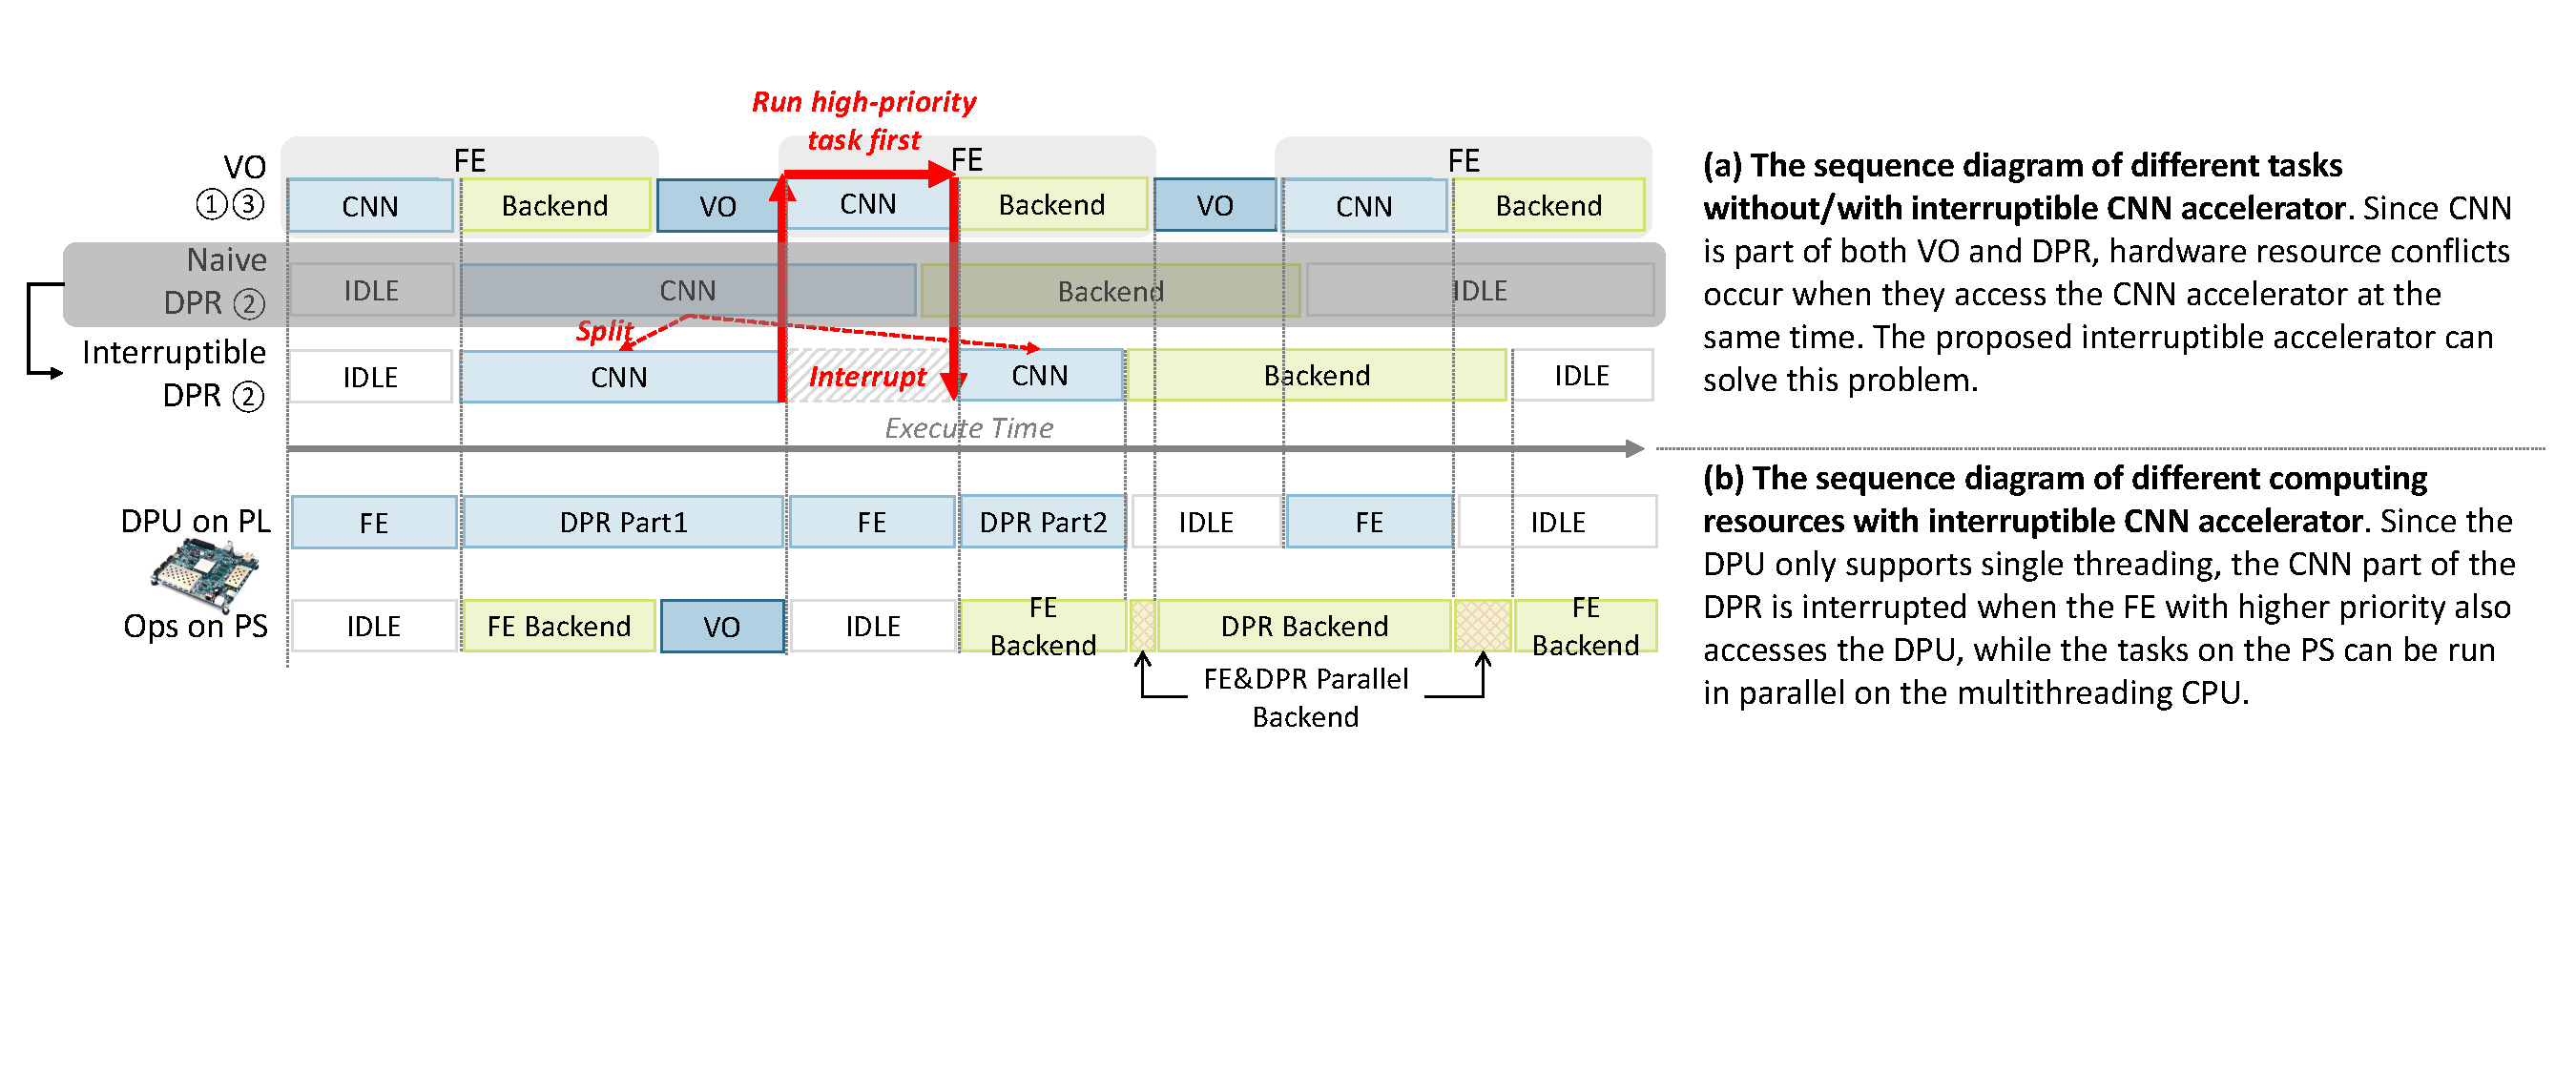
\includegraphics[width=0.99\linewidth]{fig/interDPR.pdf}
    \caption{Interruption to solve the hardware resources conflicts.  
    % When a high-priority task (FE) is started before the low-priority task (PR) is completed, the CNN accelerator backs up the status of PR to memory, and processes the FE task. When the high-priority task is completed, the low-priority task resumes and continues.
    }
	\label{fig:interDPR}
\end{figure*}


\subsection{ CNN-based FE and PR }

\textbf{\quad \ Feature-point extraction:} Previous feature-point extraction works usually consist of two parts: 1) feature-point detection to find the position of a feature-point and 2) descriptors generation to describe the extracted feature-point with a code.
SIFT \cite{Lowe-478}  detects and describes the feature-points. The SIFT descriptor is rotation and scale invariant, so that the relative pose transformation between images with matching based on SIFT is accurate. However, the computaion of SIFT is complex and slow \cite{bay2006surf}. Thus, some other handcrafted method, such as SURF\cite{bay2006surf} and ORB \cite{Mur-Artal:2017281}, are proposed as fast alternatives to SIFT. ORB \cite{Mur-Artal:2017281} method are widely used for its balance between speed and accuracy.
Recently, CNN is used to extract feature-point. \cite{simo2015discriminative} proposes a CNN-based descriptor generator that exceeds ORB in accuracy.
DeTone \cite{detone2018superpoint} presents a fully CNN-based feature-point extraction method, SuperPoint, that implements feature-point detection and descriptors generation using one CNN network. SuperPoint\cite{detone2018superpoint} reaches 10\%-30\% higher matching accuracy compared the ORB based feature-point extraction \cite{Mur-Artal:2017281} and is used in this work.

\textbf{Place recognition:} Before CNN-based place recognition, Bag of Words (BoW) \cite{small_1} relying on handcrafted features is the most popular method. The accuracy of BoW-based methods is strongly influenced by the codebook size ( descriptor length ). Larger codebooks (~1M) \cite{large_1, large_2} can compete with CNN-based methods in accuracy. However, they take up huge storage and communication resources. Smaller codebooks\cite{small_1, small_2, jegou2014triang} require less space but get worse results. In contrast to traditional methods, CNN-based methods not only perform well but also generate more compact features, saving the storage and communication resources. GeM \cite{radenovic2018fine} and NetVLAD \cite{arandjelovic2016netvlad} are popular CNN-based methods, for their accuracy and data efficiency. GeM \cite{radenovic2018fine}, is also 20\% better than the handcrafted method rootSIFT \cite{jegou2014triang}.

Due to the advantage of CNN in image-based tasks, more and more CNN-based methods are used in the robot system.


\subsection{ FPGA accelerators for a specific robot task }

The feature-point extraction (FE) operation is the basic component of a visual-based robot, and is also one of the most time consuming components \cite{fang2017fpga}.
Some previous works design hardware architectures for FE.
SRI-SURF \cite{jia2016sri} optimizes the memory access to speed up SURF \cite{bay2006surf} feature-point extraction method. 
Fang \cite{fang2017fpga} directly implements ORB on FPGA using HLS. Liu \cite{liu2019eslam} optimizes the ORB algrithm and designs a hardware for better performance.
Some other works design architectures for the entire robot system. Hero \cite{shi2018hero} is a framework for navigation and laser-based robot and cannot support visual-based robots, which is much more lightweighted and cheaper. 
Li \cite{li2019879gops} introduces CNN accelerators for the visual-based robot
However, the CNN accelerator in this work\cite{li2019879gops} is only used for feature-point extraction, and the accelerator is not to support different tasks at the same time. 
Deploying multiple CNNs on robotic accelerator can expand the functions of robots, without designing hardware for a specific function.



\subsection{ CNN accelerators }

To accelerate CNN on FPGA, some previous works design frameworks to generate a specific hardware architecture for a target CNN, based on  RTL \cite{li_high_2016} or HLS \cite{lu_evaluating_2017}. These works need to reconfigure the FPGA to switch between different CNN models. The reconfiguration comsumes seconds \cite{FPGAPerformance}, which is unacceptable for the real time system.
Some other works design instruction-driven accelerators \cite{yu2018instruction,qiu2016going,guo2017angel}, making rapid switching possible by providing different instruction sequences. 
However, the CNN tasks on previous instruction-driven CNN accelerators are not interruptible, resulting in the latency-sensitive high-priority task waiting for the low-priority task to finish. 

This inability of CNN accelerators to support multi-task makes it difficult for robotics researchers to use embedded FPGA.

% However, previous instruction-driven CNN accelerators need to schedule the entire CNN, and can not automatically schedule two or more tasks simultaneously. The inability of CNN accelerators to support multi-task makes it difficult for robotics researchers to use embedded FPGA.